\chapter{Data in organizations}
In this Chapter we discuss some high-level ideas on how databases can be
implemented in an organization. We also discuss one theoretical result that
helps to guide the choice of database implementation.


\section{Data architecture}
Understanding relational database theory and implementations thereof is one
thing. It is another thing entirely to actually use these ideas in production
environments. In practice one needs to make trade-offs between availability,
consistency, flexibility, and database performance. It has to be decided which
users have access to what data, what actions each user is allowed to perform.
For example, a data analyst may only temporarily need read-only access while
data base administrators have the ability to create or delete whole tables.
Especially in larger organisations, one needs to have procedures in place to
decide who is granted what rights, for how long, and on what grounds. 

Since there are many choices to be made, it is advantageous to have a global
overview of all things related to data in an organisation.  Such an overview is
called a 'data architecture'. To be precise, The Open Group on Architecture
Frameworks
(\hlink{https://pubs.opengroup.org/architecture/togaf9-doc/arch/index.html}{TOGAF})
defines a data architecture as follows.

\begin{terminology}{Data Architecture} 
A description of the structure and interaction of the enterprise's major types
and sources of data, logical data assets, physical data assets, and data
management resources. 
\end{terminology}
Architecture documents can describe the state of an organisation as it
currently works, but they can also serve as the design of how an organisation
should work in the future.  The idea is that this helps decision makers across
the organisation to make consistent choices. Nowadays, many large organizations
employ enterprise and data architects. For official statistics, a Common
Statistical Data Architecture was developed under the auspices of the United
Nations initiative on the modernisation of official statistics
(\hlink{https://statswiki.unece.org/display/DA}{CSDA}).

Architectures include a broad range of aspects, ranging from organizational
issues to technical (software) and physical (hardware) choices. 

In this section
we will focus on a few well-known methods for organizing databases.

As long as databases have been used in the industry, people have discussed how
to organize them. Over time, several general ideas on how to structure
databases in an organization have evolved. Many of these ideas have been
developed over time in industry, and the terminology used is not always
consistent. Most of these ideas have first been published in white papers, or
blog posts or other publications that have not been peer reviewed.  However
some of these ideas have become commonplace in industry and it is well worth
taking note of them as they do demonstrate how the theoretical ideas discussed
in Chapter~\ref{sect:relational} end up being used in practice. In the
following subsections we give an overview of some of the most well-known
database architectures, and discuss some of their advantages and disadvantages.

\subsection{Data Warehouse and Data Mart}
The data warehouse is the classical data base architecture. It is designed to
be a \emph{single source of truth} for the whole organization. This means that
the traditional data warehouse typically consists of a single database system
where all data is stored. Data that is sent to the data warehouse has to pass
strict checks before being allowed to enter. Data warehouses are governed and
centrally within an organization. Technically, they are often implemented as
relational databases. 

Data warehouses typically harbour data that is absolutely necessary to run a
business (mission-critical), and that must be consistent across the
organization. In NSIs, sampling frames that are used by various departments
fall under that category. When two sample surveys are to be used to make
inferences about the same population, the samples should be drawn from the same
population register. In businesses, customer administration and human resources
typically also fall under that category.

\begin{figure}[h]
\centering
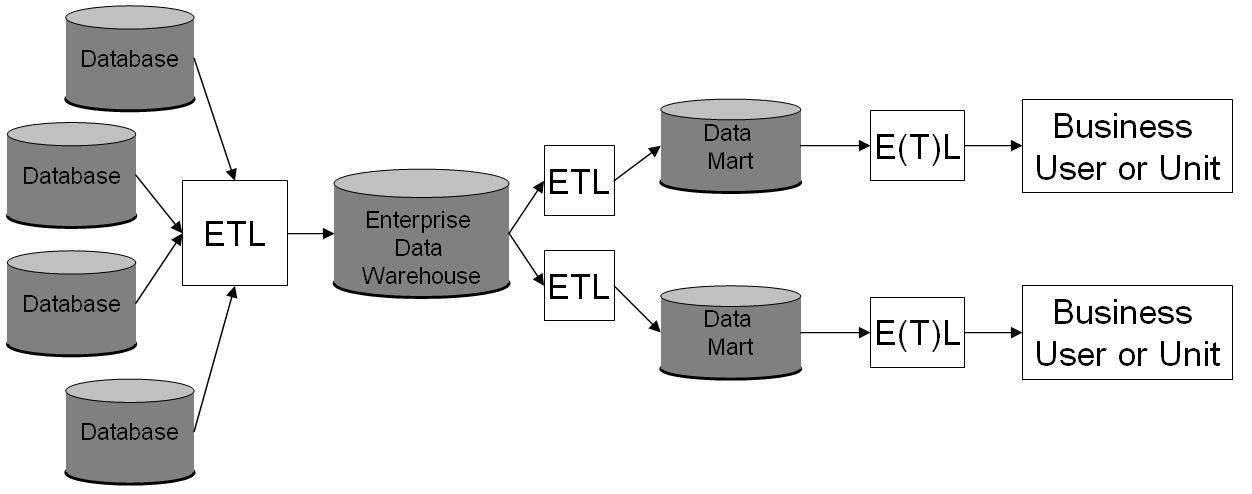
\includegraphics[height=25mm]{fig/data_warehouse_data_mart.jpg}
\caption{A data warehouse, feeding data marts. ETL stands for 
Extraction, Transformation and Loading. Picture from Wikimedia commons.}
\end{figure}

Thus, the advantage of a data warehouse architecture is that data is reliable
and strictly maintained. An immediate disadvantage is lack of flexibility.
With centrally controlled systems it may be cumbersome to create custom tables
for ad hoc analyses, or to add variables or otherwise manipulate the database
schema in ways that are interesting for analyses, since such changes
potentially have consequences in many places in the organization. 

An early answer to this disadvantage is the `data mart' architecture. In this
design, there is a central data warehouse but different users are allowed to
create their own local data bases that combine data from the warehouse with
locally created data. For example, in the case of an NSI a department that
conducts a certain business survey may join that data to a centrally stored
register of tax data and data from the Chamber of Commerce. This way, analysts
have freedom to set up local systems while the `single source of truth' stays
intact. Typical disadvantages of the data mart structure include proliferation
of data base systems and duplication of work.


\subsection{Data Lake}
The idea of a data lake was invented as an answer to the disadvantages caused
by the rigidity of centralized data warehouses. Recall that in a data
warehouse, the data base schemas are strictly controlled and therefore it may
take a lot of effort to condition data for it to be accepted into the database.
Also, as the types of data that are interesting for an organization to harvest
become more diverse and larger, keeping everything in a central data warehouse
becomes more or less impossible to organize.

The term data lake was invented by James Dixon, who wrote a blog post about it
in
\hlink{https://jamesdixon.wordpress.com/2010/10/14/pentaho-hadoop-and-data-lakes/}{2010}.
It was further elaborated upon in a white paper of \citet{stein2014enterprise}. Dixon
summarizes the idea as follows.
\begin{quote}
If you think of a datamart as a store of bottled water ---cleansed and packaged and
structured for easy consumption--- the data lake is a large body of water in a more
natural state. The contents of the data lake stream in from a source to fill the lake,
and various users of the lake can come to examine, dive in, or take samples.
\end{quote}

The idea is to remove the barrier for storing data completely. In a data lake, all
data is stored in a key-value store. Data can in principle be anything, including
documents, images, videos, audio or other formats. There is little organization
in storing the data, except for a unique identifier attached to each item. The main
task of a data lake is to store data so it can in principle be analyzed later. The
technical solution proposed by Dixon is to use a Hadoop-like key value store.

The main disadvantage of a data lake is that data needs to be gathered and
cleaned for every separate task. Having little structure in the data means that
it is hard to automate over and generally it requires more advanced skills to
work with data from a data lake than data from a data warehouse.


\subsection{Data Virtualisation}
In both the data warehouse and data lakes, data is moved from the data source
into a central or distributed database system. This may become cumbersome,
especially for very large and very diverse datasets. In data virtualisation,
data stays at the source, and instead there is a database that stores where
data can be found. Since users may access that database more or less as if it
were a regular database, this is called `data virtualisation`. The data is
retrieved by the `virtualisation' software as needed.

An advantage of data virtualisation is that the technical introduction into an
organization is relatively easy. Hardly any changes are necessary in existing
systems. The main challenges are organisational. For example in the situation
of a data mart, it needs to be decided which local databases must be connected
to the virtualisation software, and how. 



\section{The CAP theorem}
\label{sect:relational:cap}
For large datasets, data that needs to be accessed by many users, or data that
needs to be available at many places simultaneously, it is common to use some
form of distributed database. 
\begin{terminology}{Distributed database}
A distributed database is a database system that is spread over two
or more nodes.
\end{terminology}
%
The term `node' is just a fancy word for a computer in a network, or an
application that runs as if it was on a separate computer in a network. When a
database is running on multiple nodes, there has to be some communication
between the nodes to synchronize information between them. The CAP theorem
demonstrates that there are fundamental limits on what one can expect from such
a system.
%
\begin{terminology}{CAP Theorem}
A distributed database can not simultaneously be Consistent, Available, and
Partition-tolerant.
\end{terminology}
The CAP theorem was conjectured in 2002 by Eric \citet{brewer2002towards} and
proven quickly thereafter by \citet{gilbert2002brewer}.  The original proof is
a bit technical and requires a fair amount of technical definitions.  In the
current discussion we use the visual proof as discussed by
\hlink{https://mwhittaker.github.io/blog/an\_illustrated\_proof\_of\_the\_cap\_theorem/}{Whittaker},
which is easier to follow and captures the main arguments.


First consider a network composed of two nodes, called $G_1$ and $G_2$. The
network hosts a database, and both nodes have access to a stored variable with
value $v_0$.
%
\begin{center}
\begin{tikzpicture}[node distance = 2cm]
\tikzstyle{every state} = [fill=shadecolor, draw=none];
\tikzstyle{client} = [state, fill=black!20];
\tikzstyle{clnd} = [-, color=black!20];

\node[state, label=above:$G_1$] (G1) {$v_0$};
\node[client, below right of = G1, label=below:client] (cl) {};
\node[state, above right of = cl, label=above:$G_2$] (G2) {$v_0$};
\path (G1) edge (G2);
\draw[clnd] (cl) to (G1);
\draw[clnd] (cl) to (G2);

\end{tikzpicture}
\end{center}
%
The two nodes can be accessed by a client, that can request each node to return
the current value (a `read' operation) or to overwrite the current value with
another value, say $v_1$.

Now, for the database to be \textit{consistent}, means that 
\begin{quote}
any read operation that begins immediately after a write operation is completed must
return that value.
\end{quote}
The important thing is that this must hold regardless of which nodes are
receiving the read or write request. Here is how the two-node database can be
consistent: it needs to synchronizes before it is done with a `write'
operation.
\begin{center}
%% client sends 1 write request
\begin{tikzpicture}[node distance = 2cm]
  \tikzstyle{every state} = [fill=shadecolor, draw=none];
  \tikzstyle{client} = [state, fill=black!20];
  \tikzstyle{clnd} = [-, color=black!20];

  \node[state, label=above:$G_1$] (G1) {$v_0$};
  \node[client, below right of = G1, label=below:client] (cl) {};
  \node[state, above right of = cl, label=above:$G_2$] (G2) {$v_0$};
  \path (G1) edge (G2);
  \draw[clnd] (cl) to node[color=black, sloped, anchor=north, auto=false] 
                      {$\xleftarrow[\textsf{write}]{}$} (G1);
  \draw[clnd] (cl) to (G2);
\end{tikzpicture}
%% node 1 has written, and sends write request
\begin{tikzpicture}[node distance = 2cm]
  \tikzstyle{every state} = [fill=shadecolor, draw=none];
  \tikzstyle{client} = [state, fill=black!20];
  \tikzstyle{clnd} = [-, color=black!20];

  \node[state, label=above:$G_1$] (G1) {$v_1$};
  \node[client, below right of = G1, label=below:client] (cl) {};
  \node[state, above right of = cl, label=above:$G_2$] (G2) {$v_0$};
  \path (G1) edge node[above] {$\xrightarrow{\textsf{write}}$} (G2);
  \draw[clnd] (cl) to (G1);
  \draw[clnd] (cl) to (G2);
\end{tikzpicture}
%% node two has written and sends 'done' signal
\begin{tikzpicture}[node distance = 2cm]
  \tikzstyle{every state} = [fill=shadecolor, draw=none];
  \tikzstyle{client} = [state, fill=black!20];
  \tikzstyle{clnd} = [-, color=black!20];

  \node[state, label=above:$G_1$] (G1) {$v_1$};
  \node[client, below right of = G1, label=below:client] (cl) {};
    \node[state, above right of = cl, label=above:$G_2$] (G2) {$v_1$};
  \path (G1) edge (G2);
  \path (G1) edge node[above] {$\xleftarrow{\textsf{done}}$} (G2);
  \draw[clnd] (cl) to (G1);
  \draw[clnd] (cl) to (G2);
\end{tikzpicture}
%% node 1 sends 'done' signal to client.
\begin{tikzpicture}[node distance = 2cm]
  \tikzstyle{every state} = [fill=shadecolor, draw=none];
  \tikzstyle{client} = [state, fill=black!20];
  \tikzstyle{clnd} = [-, color=black!20];

  \node[state, label=above:$G_1$] (G1) {$v_1$};
  \node[client, below right of = G1, label=below:client] (cl) {};
  \node[state, above right of = cl, label=above:$G_2$] (G2) {$v_1$};
  \path (G1) edge (G2);
  \draw[clnd] (cl) to node[color=black, sloped, anchor=north, auto=false] 
                      {$\xrightarrow[\textsf{done}]{}$} (G1);
  \draw[clnd] (cl) to (G2);
\end{tikzpicture}
\end{center}
Now the client can read from either node and receive the same answer.
%
\begin{center}
\begin{tikzpicture}[node distance = 2cm]
  \tikzstyle{every state} = [fill=shadecolor, draw=none];
  \tikzstyle{client} = [state, fill=black!20];
  \tikzstyle{clnd} = [-, color=black!20];

  \node[state, label=above:$G_1$] (G1) {$v_1$};
  \node[client, below right of = G1, label=below:client] (cl) {};
  \node[state, above right of = cl, label=above:$G_2$] (G2) {$v_1$};

  \draw (G1) edge (G2);
  \draw[clnd] (cl) to (G1);
  \draw[clnd] (cl) to node[sloped, auto=false, below, text=black] {$\xrightarrow[\textsf{read}]{}$} (G2);

\end{tikzpicture}
\begin{tikzpicture}[node distance = 2cm]
  \tikzstyle{every state} = [fill=shadecolor, draw=none];
  \tikzstyle{client} = [state, fill=black!20];
  \tikzstyle{clnd} = [-, color=black!20];

  \node[state, label=above:$G_1$] (G1) {$v_1$};
  \node[client, below right of = G1, label=below:client] (cl) {};
  \node[state, above right of = cl, label=above:$G_2$] (G2) {$v_1$};

  \draw (G1) edge (G2);
  \draw[clnd] (cl) to (G1);
  \draw[clnd] (cl) to node[sloped, auto=false, below, text=black] {$\xleftarrow[v_1]{}$} (G2);

\end{tikzpicture}
\end{center}
%

The \emph{availability} demands entails the following.
\begin{quote}
every request received by a non-failing node must result in a response.
\end{quote}
This means that in an available system, if the client sends a request to a node
that is `up' (i.e. not crashed), the node must eventually return a result: nodes 
are not allowed to ignore requests.

Finally, \textit{partition-tolerance} means that
\begin{quote}
the network will be allowed to loose arbitrary many messages sent from one node to
another.
\end{quote}
In particular, partition-tolerance means that the system keeps working even
when one or more nodes are completely separated from the others.

By now, it is probably clear that the CAP theorem must hold: after all, how can
a set of nodes stay synchronized when they can not communicate write requests?
Explicitly, assume that the CAP theorem does hold and consider the situation
where $G_2$ is separated from $G_1$, so no messages can be send in either
direction.
\begin{center}
\begin{tikzpicture}[node distance = 2cm]
\tikzstyle{every state} = [fill=shadecolor, draw=none];
\tikzstyle{client} = [state, fill=black!20];
\tikzstyle{clnd} = [-, color=black!20];

\node[state, label=above:$G_1$] (G1) {$v_0$};
\node[client, below right of = G1, label=below:client] (cl) {};
\node[state, above right of = cl, label=above:$G_2$] (G2) {$v_0$};
\draw[clnd] (cl) to (G1);
\draw[clnd] (cl) to (G2);

\end{tikzpicture}
\end{center}
%
The client sends a write request. Because Availability is assumed, $G_1$ must
answer.
\begin{center}
%% client sends 1 write request
\begin{tikzpicture}[node distance = 2cm]
  \tikzstyle{every state} = [fill=shadecolor, draw=none];
  \tikzstyle{client} = [state, fill=black!20];
  \tikzstyle{clnd} = [-, color=black!20];

  \node[state, label=above:$G_1$] (G1) {$v_0$};
  \node[client, below right of = G1, label=below:client] (cl) {};
  \node[state, above right of = cl, label=above:$G_2$] (G2) {$v_0$};
  
  \draw[clnd] (cl) to node[color=black, sloped, anchor=north, auto=false] 
                      {$\xleftarrow[\textsf{write}]{}$} (G1);
  \draw[clnd] (cl) to (G2);
\end{tikzpicture}
%% node 1 sends 'done' signal to client.
\begin{tikzpicture}[node distance = 2cm]
  \tikzstyle{every state} = [fill=shadecolor, draw=none];
  \tikzstyle{client} = [state, fill=black!20];
  \tikzstyle{clnd} = [-, color=black!20];

  \node[state, label=above:$G_1$] (G1) {$v_1$};
  \node[client, below right of = G1, label=below:client] (cl) {};
  \node[state, above right of = cl, label=above:$G_2$] (G2) {$v_0$};
  \draw[clnd] (cl) to node[color=black, sloped, anchor=north, auto=false] 
                      {$\xrightarrow[\textsf{done}]{}$} (G1);
  \draw[clnd] (cl) to (G2);
\end{tikzpicture}
\end{center}
The consistency demand is now violated, since reading from $G_2$ does not
return the value written by the last completed write operation.
\begin{center}
\begin{tikzpicture}[node distance = 2cm]
  \tikzstyle{every state} = [fill=shadecolor, draw=none];
  \tikzstyle{client} = [state, fill=black!20];
  \tikzstyle{clnd} = [-, color=black!20];

  \node[state, label=above:$G_1$] (G1) {$v_1$};
  \node[client, below right of = G1, label=below:client] (cl) {};
  \node[state, above right of = cl, label=above:$G_2$] (G2) {$v_0$};

  \draw[clnd] (cl) to (G1);
  \draw[clnd] (cl) to node[sloped, auto=false, below, text=black] {$\xrightarrow[\textsf{read}]{}$} (G2);

\end{tikzpicture}
\begin{tikzpicture}[node distance = 2cm]
  \tikzstyle{every state} = [fill=shadecolor, draw=none];
  \tikzstyle{client} = [state, fill=black!20];
  \tikzstyle{clnd} = [-, color=black!20];

  \node[state, label=above:$G_1$] (G1) {$v_1$};
  \node[client, below right of = G1, label=below:client] (cl) {};
  \node[state, above right of = cl, label=above:$G_2$] (G2) {$v_0$};

  \draw[clnd] (cl) to (G1);
  \draw[clnd] (cl) to node[sloped, auto=false, below, text=black] {$\xleftarrow[v_0]{}$} (G2);

\end{tikzpicture}
\end{center}
In conclusion, assuming consistency, availability and partition-tolerance leads
to a contradiction. The above example demonstrates that a partitioned network
can not host a database that is both available and consistent.

\section{Practical consequences of the CAP theorem}
Since the CAP theorem tells us that we can't have partition tolerance while
being consistent and available, this means we need to choose what is most
important for a certain application. Let us discuss a few ways in which
different types of database systems (CA, CP, or AP) can be implemented.



\subsection{Consistent, Available}
A partition-tolerant system can be created by using a single storage
facility. The architecture looks like in Figure~\ref{fig:ca}.
\begin{figure}
\centering
\begin{tikzpicture}[node distance = 2cm]
  \tikzstyle{every state} = [fill=shadecolor, draw=none];
  \tikzstyle{client} = [state, fill=black!20];
  \tikzstyle{clnd} = [-, color=black!20];

  \node[state, label=above:server] (server) {};
  \node[client, below left of = server, label=below:client] (cl1) {};
  \node[client, below  of = server, label=below:client] (cl2) {};
  \node[client, below right of = server, label=below:client] (cl3) {};

  \draw[clnd] (cl1) to (server);
  \draw[clnd] (cl2) to (server);
  \draw[clnd] (cl3) to (server);

\end{tikzpicture}
\caption{Consistent and available: all data on a single node.}
\label{fig:ca}
\end{figure}
There are one or more clients that send requests to a single data storage node.
Requests are handled in order of arrival by the server and a new request is not
handled until the previous one has been completed.  We have consistency since
no synchronisation needs to take place, and since every request to a
non-failing node (a single server node here) will indeed yield a response. The
idea of partition-tolerance becomes irrelevant in this architecture since there
are no data storage nodes to partition by breaking links between them.

The point is that if you want a system that is 100\% Consistent and Available,
you are forced to create a centralized system. Many traditional transactional
database solutions are built this way.

\subsection{Consistent, Partition-tolerant}
Here, we drop availability. The simplest solution for creating a database that
is both consistent and partition tolerant is by building a system where every
node ignores every request. This means that every read operation receives the
same answer: none. It is also partition-tolerant since all nodes always behave
the same and no synchronisation is necessary.

More realistically, a master node can be appointed to distribute data across
nodes, and to queue requests from clients. A read operation cannot take place
before the last write operation is fully complete across all nodes. This means
that when one client issues a request, the others have to wait. An example of
such architecture is shown in Figure~\ref{fig:cp}.
\begin{figure}[h]
\centering
\begin{tikzpicture}[node distance = 2cm]
  \tikzstyle{every state} = [fill=shadecolor, draw=none];
  \tikzstyle{client} = [state, fill=black!20];
  \tikzstyle{clnd} = [-, color=black!20];

  \node[state, label=right:master] (master) {};
  \node[state, above left of = master, label=above:server] (sv1) {1};
  \node[state, above  of = master, label=above:server] (sv2) {2};
  \node[state, above  right of = master, label=above:server] (sv3) {3};
  \node[client, below left of = master, label=below:client] (cl1) {};
  \node[client, below  of = master, label=below:client] (cl2) {};
  \node[client, below right of = master, label=below:client] (cl3) {};

  \draw[clnd] (cl1) to (master);
  \draw[clnd] (cl2) to (master);
  \draw[clnd] (cl3) to (master);
  \draw[clnd] (master) to (sv1);
  \draw[clnd] (master) to (sv2);
  \draw[clnd] (master) to (sv3);


\end{tikzpicture}
\caption{Consistent and partition-tolerant: a single node handles all requests.}
\label{fig:cp}
\end{figure}
Now, if the connection between the master node and server 1 is severed, then
any request that would involve reading from or writing to server 1 will be
dropped (loss of availability). The data that is still reachable on servers 2
and 3 is still consistent across read/write requests.  Such problems can
be avoided by partially duplicating data across servers. An example of this is
Hadoop/HBase. Here, a central node distributes data across multiple nodes.
All data is written to say, three out of $n$ nodes. This means that
availability is only compromised when all three servers that hold a certain
value become unreachable. In practice the probability of such an event may be
low but in terms of the CAP theorem it does mean dropping the Availability
property.

\subsection{Available and Partition-tolerant}
Here we drop the demand that a read request always returns the latest write
result. In Figure~\ref{fig:ap}, a client may write something to one node and
request a value from another node before the write operation has spread across
the network. Or, client 1 may write something to server 1, and client 2 reads
the same information from server 3 before the nodes have synchronized. 
\begin{figure}[h]
\centering
\begin{tikzpicture}[node distance = 2cm]
  \tikzstyle{every state} = [fill=shadecolor, draw=none];
  \tikzstyle{client} = [state, fill=black!20];
  \tikzstyle{clnd} = [-, color=black!20];

  \node[] (center) {};
  \node[client,left of = center, label=below:client] (lclient) {1};
  \node[client,right of = center, label=below:client] (rclient) {2};
  \node[state, above left of = center, label=above:server] (sv1) {1};
  \node[state, above  of = center, label=above:server] (sv2) {2};
  \node[state, above  right of = center, label=above:server] (sv3) {3};

  \draw[clnd] (lclient) to (sv1);
  \draw[clnd] (lclient) to (sv2);
  \draw[clnd] (lclient) to (sv3);
  \draw[clnd] (rclient) to (sv1);
  \draw[clnd] (rclient) to (sv2);
  \draw[clnd] (rclient) to (sv3);
  \draw[clnd] (sv1) to (sv2);
  \draw[clnd] (sv1) to (sv3);
  \draw[clnd] (sv2) to (sv3);

\end{tikzpicture}
\caption{Available and partition-tolerant: there's always a node that answers,
but the servers may not have synchronized information.}
\label{fig:ap}
\end{figure}
An example of such behavior is in social media or online search engines
(Google) where users from different locations may not always get the same
search result at the same time (of course such differences are also obscured by
personalisation).



\section*{Where are we?}
We have seen that there are a few main architectural paradigms on organizing
data in large organizations. These paradigms are based on, and evolve with
practical experience and increasing technological capabilities. The CAP theorem
is a theoretical result that forces one to decide between consistency,
availability or partition-tolerance of a distributed database.


\section{Exercises}
\begin{enumerate}
\item Go to the TOGAF website, and read the
\hlink{https://pubs.opengroup.org/architecture/togaf9-doc/arch/chap01.html\#tag\_01\_03}{Executive
Overview}. Pay attention to how the term `enterprise' is defined.

\item Look up the entries of Data Warehouse, Data Mart, Data Lake,
and Data Virtualisation on Wikipedia. Create a table with pro's and cons
in the columns and an architecture on each row.
\item Using the same system as in Section~\ref{sect:relational:cap},
demonstrate that a distributed database that does not satisfy the availability
condition can be consistent and partition-tolerant. Tips: consider nodes that
can send a `fail' message when they find out that a `write' message is lost.

\item Below are three fictional cases. In this assignment, students are grouped
in teams of 3-5 students. 


Discuss, in about 20-30 minutes, which of the four architectural patterns: Data
Warehouse (DW), Data Mart (DM), Data Lake (DL) or Data Virtualization (DV)
would be preferred. Consider things like the CAP requirements, and realize that
it may be possible to combine strategies. If you have questions about details
in the example just make a reasonable assumption. Feel free to read online
blogs/opinions by data architects for inspiration, or dig up the definitions on
e.g. Wikipedia.


Each team will give a presentation of about 5 minutes, covering the following aspects.
\begin{enumerate}
\item Type of organization as defined in the above description.
\item The choice you made: DW, DM, DL, DV? and
\item most importantly: why you made this choice.
\end{enumerate}
\end{enumerate}


\begin{subappendices}
\section{Cases}
\subsection{The startup}

You work for a fast-growing online startup called `Borkly'. Their product is a
\emph{Next-Generation Search Engine for Old People} with a freemium business model:
customers either use the service for free with adds or choose to take an
add-free subscription with monthly payments. The company works remote-first, so
almost everybody works from home. There are currently 40 people in the company
(not all of them full-time): 3 owner/managers, 22 developers, 5 data analysts
and 10 customer support employees.

For their growing customer support department they are looking to replace their
current ad hoc customer administration (CRM) database backend. The current
system is slow, buggy, and even some simple administrative activities sometimes
take a lot of 'manual' work. There are really only two people who understand how
it works. At the moment Borkly only stores the bare necessities to keep
administration going. In the future they want to be able to store everything
they can get from every customer, including site visits/audit trails, e-mails,
and so on, to be able to serve their data analysts with information.



\subsection{The statistical office}

You work for the \emph{Center of Statistical Information for the Country}. This
bureau is responsible for collecting, producing, and publishing, all national
statistics. It is an organization with about 1000 employees, who all work in the
same building. Although there is one organization, historically each statistical
domain collected and processed its own data, leading to a broad and varying
landscape of data storage solutions, varying from text-files (csv) to
professional data bases. Although such solutions are locally optimal (i.e. they
can be maintained by the departments using them, with some help from the IT
department), management feels that some form of unification would benefit the
Center as a whole.

In the future, the organization would like to cut costs by removing overlapping
information from the organization. They would also like to develop new,
frequently published, statistical products based on the combination of various
data streams in the Center. They would also like data analysts to be able to
quickly create one-off on-demand analysis for external customers. Finally, they
would like to leverage the large quantities of information coming from the
internet of things (IoT) such as mobile phone data for their statistical
products.


\subsection{The government}

You work at the National Office of Employment. This office is responsible for
registering the unemployed, and for payment of unemployment benefits.
Historically, the office was created by merging several regional offices with a
similar task. Although there have been some attempts to unify the legacy data
warehouses into a single data warehouse, the differences between storage
solutions and (meta)data are so large that the office in some respects works
more like a cluster of local offices than as a single unified entity.

The NOE's board recently decided that fraud detection is a spear point within
the organization. To do this it is necessary to integrate both existing data
sources, and new external sources, for example tax records and sometimes social
media records from suspects. The data analyses department is given extra budget
to hire data scientists and they are now talking to the IT department on how to
shape the data landscape.



\end{subappendices}






